
\section{Thursday}\index{Thursday_lecture}
\subsection{Examples}
Minimal surface equation.\\
Given a curve $\Gamma$ in $\mathbb{R}^3$ to find a surface spanning $\Gamma$ and has the smallest possible area.
\[(1+u_y^2)u_{xx}-2u_xu_yu_{xy}+(1+u_x^2)u_{yy}=0
\]
This is a $\second$ order linear in $\uxx,\uyy$ equation. It is called quasi-linear equation.\\
Now, before we take a look at solving some partial differential equations. Let's review a simple ode case.\\
In ODE,
\[v\p+cv=0
\]
\[\frac{\diff v}{\diff t}=v\p=-cv
\]
\[\frac{\diff v}{v}=-c\diff t
\]
At the moment, just ignore $|v|$
\[\ln v=-ct+\alpha
\]
\[v(t)=e^{-ct}e^\alpha=v(0)e^{-ct}, t=0~ v(0)=e^\alpha
\]
In PDE,
\[\uy+c\ux=0 ~c\text{: constant}
\]
This is called transport equation. Later on, we will talk about this name.
\[\deriva{t}u(x(t),y(t))=u_x\deriv{x}{t}+\uy\deriv{y}{t}=c\ux+\uy=0
\]
\[\left\{\begin{gathered}\deriv{x}{t}=c\\\deriv{y}{t}=1\end{gathered}\right.~\Rightarrow~\left\{\begin{gathered}x=ct+X(0)=ct+\xi\\y=t+y(0)=t\end{gathered}\right.
\]
\[\Rightarrow \xi=x-ct\qquad\xi=x-cy\]
On $\Gamma_\xi$, $\deriv{t}u(x(t),y(t))\equiv0$ $\forall t \Rightarrow$, $u(x(t),y(t))\equiv$ constant on $\Gamma_\xi$.\\
\[u(x,y)=f(x-cy)
\]
As convention, let $t$ denote $y$, transport equation is $\begin{cases}u_t+c\ux=0\\u(x,0)=f(x)\end{cases}~\Rightarrow~u(x,t)=f(x-ct)$.\\
The following is a graph used to illustrate why it is called transport equation:
\[u(cT,T)=f(cT-cT)=f(0)=u(0,0)
\]
\begin{figure}[H]
\centering
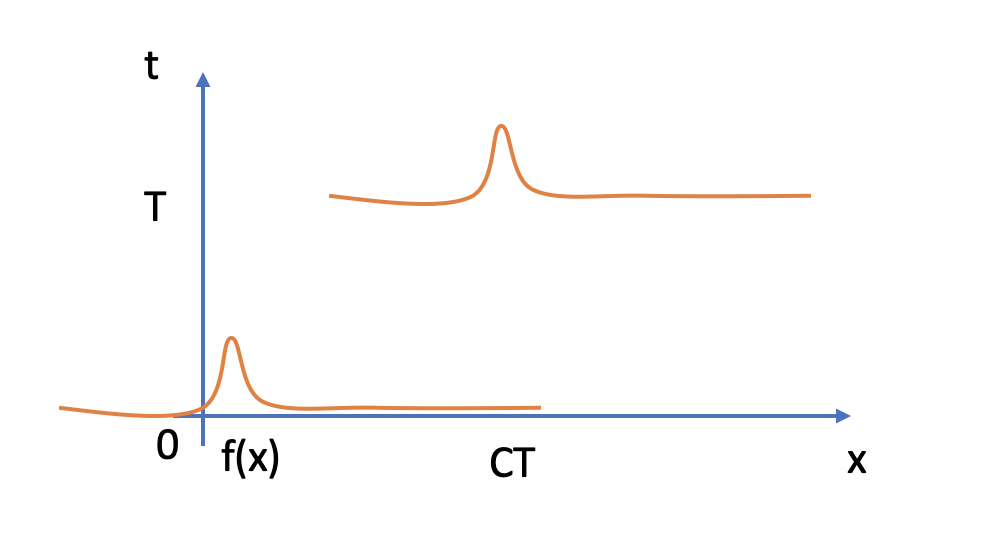
\includegraphics[width=10cm]{week1_thursday1}
\end{figure}
\begin{example}
\[\left \{\begin{gathered}x\ux+y\uy=\alpha u\\u(x,1)=f(x)\end{gathered}\right.
\]
$\Gamma:$ characteristic curve $\dakuohao{\deriv{x}{t}=x}{\deriv{y}{t}=y}~\Rightarrow~\dakuohao{x=x_0e^t=se^t}{y=y_0e^t=1e^t~\rightarrow~t=\ln y}$.\\
Initial curve $\dakuohao{x=s}{y=1}$.\\
\[s=\frac{x}{e^t}=\frac{x}{y}
\]
On $\Gamma$, we have $\deriv{u}{t}=\ux\deriv{x}{t}+\uy\deriv{y}{t}=x\ux+y\uy=\alpha u\Rightarrow u=ce^{\alpha t}=f(s)e^{\alpha}$
About the last equal sign of above equation, it is because $u(x_0,y_0)=u(s,1)=c$ when t=0.
\[u(x,y)=f(\frac{x}{y})y^\alpha
\]


\end{example}
Next lecture will discuss quasi-linear equation.
\[a(x,y,u)\ux+b(x,y,u)\uy=c(x,y,u)
\]


